\documentclass[aspectratio=169,11pt,xcolor=table]{beamer}

\usepackage[T1]{fontenc}
\usepackage[utf8]{inputenc}
\usepackage{helvet}
\usepackage{graphicx}
\usepackage{booktabs}
\usepackage{tabularx}
\usepackage{array}
\usepackage{ragged2e}
\usepackage{hyperref}

\renewcommand{\familydefault}{\sfdefault}
\graphicspath{{assets/}}
\urlstyle{same}

\definecolor{Canvas}{HTML}{FFFFFF}
\definecolor{Ink}{HTML}{111827}
\definecolor{Muted}{HTML}{667085}
\definecolor{Panel}{HTML}{EEF1F5}
\definecolor{Rule}{HTML}{B8BCC4}
\definecolor{Accent}{HTML}{3D8DFF}
\definecolor{AccentLight}{HTML}{DCEEFF}
\definecolor{Good}{HTML}{168B5B}
\definecolor{GoodLight}{HTML}{E1F3EA}
\definecolor{Warn}{HTML}{E66A2C}
\definecolor{WarnLight}{HTML}{FBE8DE}
\definecolor{Purple}{HTML}{7452C8}

\setbeamercolor{background canvas}{bg=Canvas}
\setbeamercolor{normal text}{fg=Ink,bg=Canvas}
\setbeamercolor{frametitle}{fg=Ink,bg=Canvas}
\setbeamercolor{structure}{fg=Accent}
\setbeamercolor{alerted text}{fg=Warn}
\setbeamercolor{block title}{fg=Ink,bg=Panel}
\setbeamercolor{block body}{fg=Ink,bg=Panel}

\setbeamerfont{normal text}{size=\fontsize{11.4}{13.7}\selectfont}
\setbeamerfont{frametitle}{size=\fontsize{20}{23}\selectfont,series=\bfseries}
\setbeamerfont{title}{size=\fontsize{26}{30}\selectfont,series=\bfseries}
\setbeamerfont{subtitle}{size=\fontsize{12.5}{15}\selectfont}
\setbeamerfont{block title}{size=\fontsize{13.5}{16}\selectfont,series=\bfseries}
\setbeamerfont{block body}{size=\fontsize{10.8}{13}\selectfont}

\setbeamertemplate{navigation symbols}{}
\setbeamertemplate{itemize item}{\color{Accent}\raise0.18ex\hbox{\rule{0.55ex}{0.55ex}}}
\setbeamertemplate{itemize subitem}{\color{Accent}\raise0.18ex\hbox{\rule{0.42ex}{0.42ex}}}
\setbeamertemplate{frametitle}{%
  \vspace{0.20cm}%
  \begin{beamercolorbox}[wd=\paperwidth,leftskip=0.62cm,rightskip=0.62cm]{frametitle}%
    \usebeamerfont{frametitle}\insertframetitle\par%
    \vspace{0.10cm}%
    {\color{Rule}\rule{\dimexpr\paperwidth-1.24cm\relax}{0.45pt}}%
  \end{beamercolorbox}%
}
\setbeamertemplate{footline}{%
  \leavevmode%
  \hbox{%
    \begin{beamercolorbox}[wd=.82\paperwidth,ht=0.34cm,dp=0.13cm,leftskip=0.62cm]{author in head/foot}%
      {\color{Muted}\fontsize{6.7}{8}\selectfont Trust-aware connected vehicle project}%
    \end{beamercolorbox}%
    \begin{beamercolorbox}[wd=.18\paperwidth,ht=0.34cm,dp=0.13cm,rightskip=0.62cm plus1fil]{date in head/foot}%
      {\color{Muted}\fontsize{6.7}{8}\selectfont\hfill\insertframenumber/\inserttotalframenumber}%
    \end{beamercolorbox}%
  }%
}
\setbeamertemplate{blocks}[default]
\setbeameroption{hide notes}

\newcommand{\eyebrow}[1]{%
  {\color{Accent}\fontsize{7.5}{9}\selectfont\bfseries\MakeUppercase{#1}}\par\vspace{0.14cm}%
}
\newcommand{\sourcefoot}[1]{%
  % Provenance is retained in each frame's hidden [Sources] speaker note.
}
\newcommand{\metric}[2]{%
  {\color{Accent}\fontsize{20}{22}\selectfont\bfseries #1}\par%
  \vspace{0.06cm}{\fontsize{8.8}{10.6}\selectfont #2}%
}
\newcommand{\quietmetric}[2]{%
  {\color{Ink}\fontsize{15.5}{18}\selectfont\bfseries #1}\par%
  \vspace{0.04cm}{\color{Muted}\fontsize{8.5}{10.2}\selectfont #2}%
}
\newcommand{\stepnumber}[1]{%
  {\color{Accent}\fontsize{18}{20}\selectfont\bfseries #1}%
}

\title{Trust-aware resilience for connected vehicle platoons}
\subtitle{From attack-aware state estimation to an onboard edge module}
\author{Quang Huy Nguyen}
\institute{CRAN - Universite de Lorraine / SEGULA Engineering}
\date{Project overview - 2026}

\begin{document}

% -----------------------------------------------------------------------------
\begin{frame}[plain]
  \begin{columns}[T,totalwidth=\paperwidth]
    \begin{column}{0.56\paperwidth}
      \vspace{0.75cm}
      \hspace{0.68cm}\begin{minipage}{0.48\paperwidth}
        \raggedright\hyphenpenalty=10000\exhyphenpenalty=10000
        \eyebrow{Connected vehicle cyber-resilience}
        {\color{Ink}\fontsize{20.5}{24}\selectfont\bfseries
          Trust-aware resilience\par
          for connected\par
          vehicle platoons\par}
        \vspace{0.32cm}
        {\usebeamerfont{subtitle}\color{Muted}\insertsubtitle\par}
        \vspace{0.62cm}
        {\fontsize{9.5}{11.5}\selectfont Project overview for potential users and decision-makers\par}
        \vspace{0.22cm}
        {\color{Muted}\fontsize{8.2}{10}\selectfont Quang Huy Nguyen - CRAN / SEGULA Engineering}
      \end{minipage}
    \end{column}
    \begin{column}{0.44\paperwidth}
      \color{Accent}\rule{0.12cm}{\paperheight}\hspace{0.12cm}%
      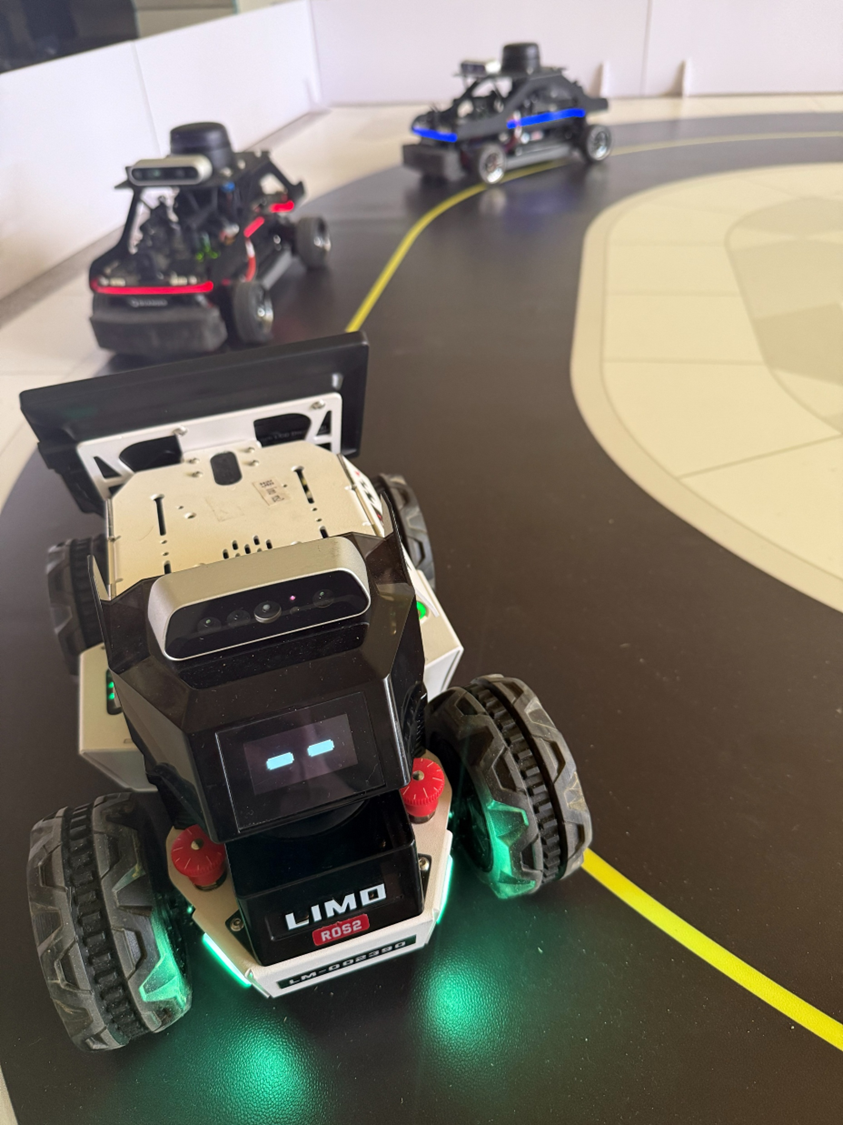
\includegraphics[height=0.91\paperheight,width=0.39\paperwidth,keepaspectratio]{qcar_limo.png}
    \end{column}
  \end{columns}
  \note{[Sources]\par
    Project title and authorship: \texttt{\detokenize{manuscript_v7_submit.tex}}.\par
    Image: \texttt{\detokenize{ch5/TRust_final/img/image.png}} (user-provided project asset).}
\end{frame}

% -----------------------------------------------------------------------------
\begin{frame}{Connectivity creates physical risk}
  \eyebrow{Context}
  {\fontsize{16}{19}\selectfont\bfseries Cooperative driving depends on data the vehicle cannot fully trust.\par}
  \vspace{0.20cm}
  {\fontsize{9.7}{11.7}\selectfont
  \begin{columns}[T,onlytextwidth]
    \begin{column}{0.47\textwidth}
      {\color{Good}\fontsize{13}{15}\selectfont\bfseries What connectivity enables}\par
      \vspace{0.17cm}
      \begin{itemize}
        \item Shared position, speed, heading and acceleration
        \item Cooperative cruise control and coordinated platoons
        \item Smoother traffic flow with fewer onboard measurements
      \end{itemize}
    \end{column}
    \begin{column}{0.47\textwidth}
      {\color{Warn}\fontsize{13}{15}\selectfont\bfseries What an attack can change}\par
      \vspace{0.17cm}
      \begin{itemize}
        \item False, replayed, delayed or missing V2V packets
        \item Corrupted estimates that propagate across the fleet
        \item Unsafe control decisions based on plausible-looking data
      \end{itemize}
    \end{column}
  \end{columns}}
  \vspace{0.16cm}
  \begin{beamercolorbox}[sep=0.14cm,wd=\textwidth]{block body}
    \fontsize{9.2}{11}\selectfont\bfseries Preserve cooperative value; degrade safely when V2V evidence is unreliable.
  \end{beamercolorbox}
  \sourcefoot{Final trust-observer manuscript, Introduction and threat model}
  \note{[Sources]\par
    \texttt{\detokenize{ch5/TRust_final/manuscript_v7_submit.tex}}, Introduction and Problem formulation and threat model.}
\end{frame}

% -----------------------------------------------------------------------------
\begin{frame}{A trust layer protects cooperation}
  \eyebrow{Project concept}
  \centering
  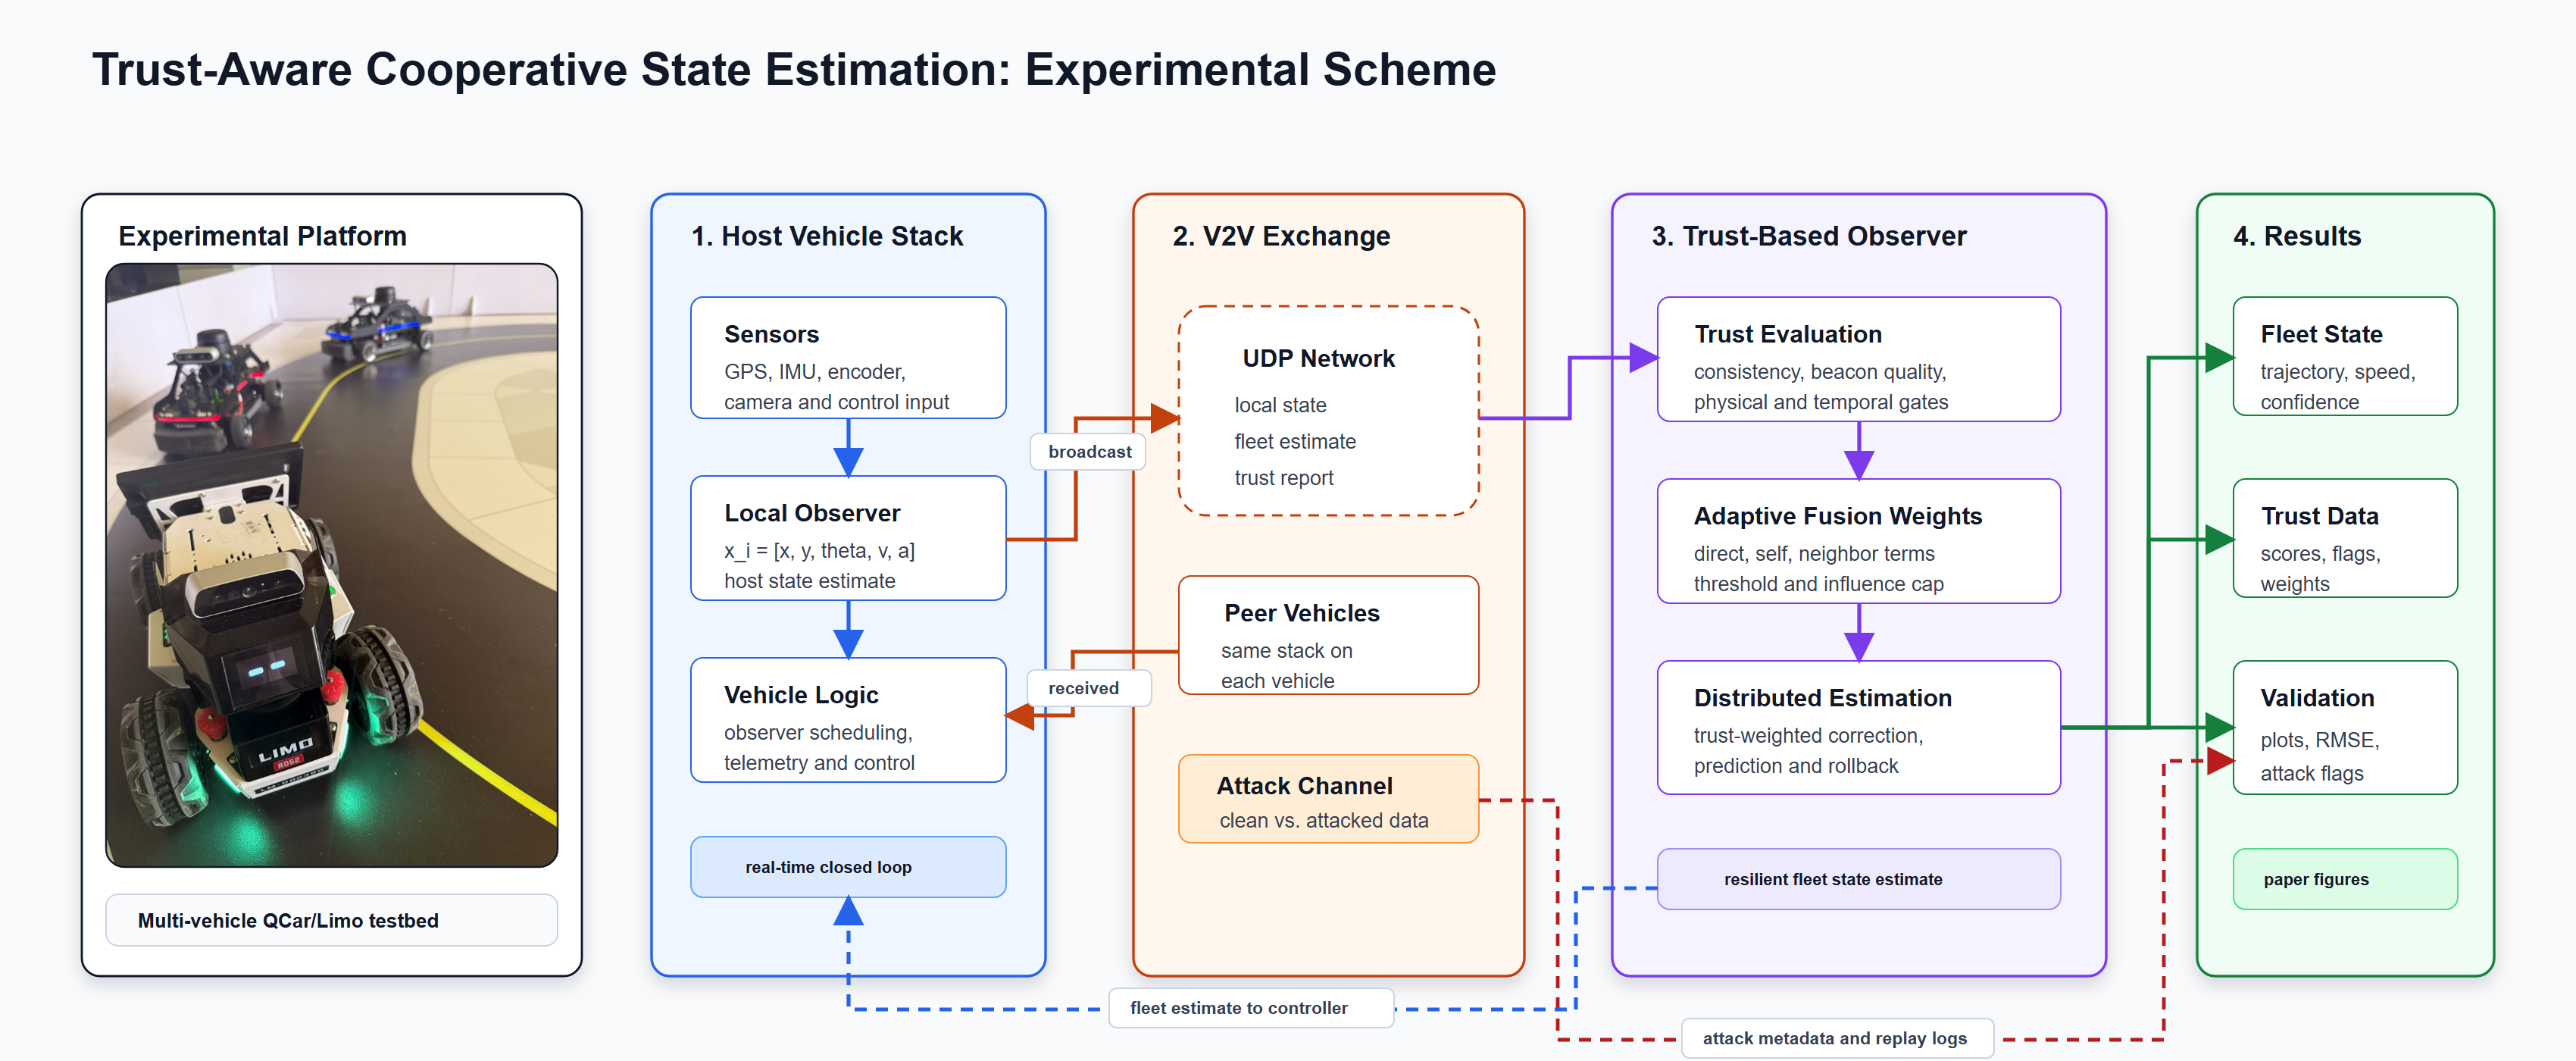
\includegraphics[width=0.92\textwidth,height=0.49\textheight,keepaspectratio]{experimental_scheme.png}
  \vspace{0.06cm}
  \begin{beamercolorbox}[sep=0.12cm,wd=0.94\textwidth]{block body}
    \centering\fontsize{9.2}{11}\selectfont\bfseries The trust layer screens, weighs and corrects data before the existing controller.
  \end{beamercolorbox}
  \sourcefoot{Final trust-observer manuscript and project experimental-scheme figure}
  \note{[Sources]\par
    \texttt{\detokenize{ch5/TRust_final/manuscript_v7_submit.tex}}, QCar/LIMO platform and communication stack.\par
    Image: \texttt{\detokenize{ch5/img/global_system_scheme_ieee_simple.png}} (user-provided project asset).}
\end{frame}

% -----------------------------------------------------------------------------
\begin{frame}{Board sits at the data-control boundary}
  \eyebrow{Electronic board integration}
  \begin{columns}[T,onlytextwidth]
    \begin{column}{0.28\textwidth}
      {\color{Accent}\fontsize{11.5}{13.5}\selectfont\bfseries Inputs}\par
      \vspace{0.13cm}
      {\fontsize{9.3}{11.2}\selectfont
      \begin{itemize}
        \item IMU and local kinematics
        \item GNSS position and 1PPS timing
        \item Vehicle-bus data and V2V packets: Wi-Fi now, C-V2X later
      \end{itemize}}
    \end{column}
    \begin{column}{0.07\textwidth}
      \vspace{1.35cm}\centering{\color{Rule}\fontsize{24}{26}\selectfont$\Rightarrow$}
    \end{column}
    \begin{column}{0.30\textwidth}
      {\color{Purple}\fontsize{11.5}{13.5}\selectfont\bfseries Edge functions}\par
      \vspace{0.13cm}
      {\fontsize{9.3}{11.2}\selectfont
      \begin{itemize}
        \item Time and packet-validity gates
        \item State estimation, trust and source weighting
        \item Rollback, re-anchoring and audit logs
      \end{itemize}}
    \end{column}
    \begin{column}{0.07\textwidth}
      \vspace{1.35cm}\centering{\color{Rule}\fontsize{24}{26}\selectfont$\Rightarrow$}
    \end{column}
    \begin{column}{0.28\textwidth}
      {\color{Good}\fontsize{11.5}{13.5}\selectfont\bfseries Outputs}\par
      \vspace{0.13cm}
      {\fontsize{9.3}{11.2}\selectfont
      \begin{itemize}
        \item Trusted state estimates
        \item Attack, trust, availability and health flags
        \item CAN/CAN-FD or gateway data for controller and planner
      \end{itemize}}
    \end{column}
  \end{columns}
  \vspace{0.22cm}
  \begin{beamercolorbox}[sep=0.14cm,wd=\textwidth]{block body}
    \fontsize{9.2}{11}\selectfont\textbf{Integration principle:} start in monitoring mode; introduce control authority only after timing, robustness and safety gates are demonstrated.
  \end{beamercolorbox}
  \sourcefoot{Thesis Chapter 6, board motivation, functional requirements and integration roadmap}
  \note{[Sources]\par
    \texttt{\detokenize{ch6/ch6_main.tex}}, Custom embedded electronic board for future onboard deployment, component selection, firmware structure and integration roadmap.}
\end{frame}

% -----------------------------------------------------------------------------
\begin{frame}{Intervention is graduated, not binary}
  \eyebrow{Response when an attack is detected}
  \vspace{0.08cm}
  {\fontsize{9.2}{11}\selectfont
  \begin{tabularx}{\textwidth}{>{\centering\arraybackslash}X c >{\centering\arraybackslash}X c >{\centering\arraybackslash}X c >{\centering\arraybackslash}X c >{\centering\arraybackslash}X}
    {\color{Good}\bfseries Accept} & $\rightarrow$ &
    {\color{Accent}\bfseries Down-weight} & $\rightarrow$ &
    {\color{Warn}\bfseries Isolate} & $\rightarrow$ &
    {\color{Purple}\bfseries Correct} & $\rightarrow$ &
    {\color{Ink}\bfseries Fallback} \\
    \rule{0pt}{0.45cm}fresh, plausible packet && inconsistent neighbor loses influence && attacked source weight becomes zero && rollback and anchoring repair recent state && trust gate shifts CACC toward local ACC
  \end{tabularx}}
  \vspace{0.34cm}
  \begin{beamercolorbox}[sep=0.18cm,wd=\textwidth]{block body}
    \fontsize{9.5}{11.4}\selectfont\textbf{Two complementary effects:} rejection stops future influence; rollback and anchoring revise recent contamination.
  \end{beamercolorbox}
  \vspace{0.18cm}
  {\color{Warn}\fontsize{9}{10.8}\selectfont\bfseries Current scope:} {\fontsize{9}{10.8}\selectfont the prototype does not claim direct actuator override; the vehicle controller retains command authority.}
  \sourcefoot{Final trust-observer manuscript, packet gate, rollback and trust-gated ACC/CACC}
  \note{[Sources]\par
    \texttt{\detokenize{ch5/TRust_final/manuscript_v7_submit.tex}}, packet validity gate, Contamination rollback, and Distributed state estimation for platoon control.\par
    \texttt{\detokenize{ch6/ch6_main.tex}}, integration roadmap and safe degradation modes.}
\end{frame}

% -----------------------------------------------------------------------------
\begin{frame}{Validation moved from model to hardware}
  \eyebrow{Work performed}
  \centering
  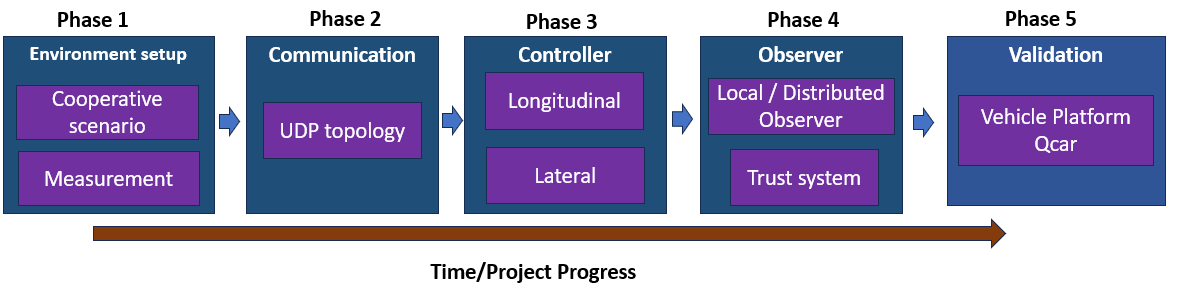
\includegraphics[width=0.86\textwidth,height=0.28\textheight,keepaspectratio]{validation_phases.png}
  \vspace{0.03cm}
  \begin{columns}[T,onlytextwidth]
    \begin{column}{0.31\textwidth}
      {\fontsize{10}{11.8}\selectfont\bfseries 1. Numerical campaign}\par
      {\color{Muted}\fontsize{7.7}{9.2}\selectfont Five vehicles, controlled ground truth and multi-channel attacks.}
    \end{column}
    \begin{column}{0.31\textwidth}
      {\fontsize{10}{11.8}\selectfont\bfseries 2. Digital twin and scale models}\par
      {\color{Muted}\fontsize{7.7}{9.2}\selectfont QLabs + QCar/LIMO: packets, timing and closed-loop paths.}
    \end{column}
    \begin{column}{0.31\textwidth}
      {\fontsize{10}{11.8}\selectfont\bfseries 3. Embedded transfer}\par
      {\color{Muted}\fontsize{7.7}{9.2}\selectfont PCB: RTOS, sensors, radio, timing and logging.}
    \end{column}
  \end{columns}
  \sourcefoot{Thesis Chapter 6 experimental methodology; final manuscript validation layers}
  \note{[Sources]\par
    \texttt{\detokenize{ch6/ch6_main.tex}}, Experimental methodology: from virtual validation to real trials.\par
    Image: \texttt{\detokenize{ch6/fig/Modular_Experimental_Phases.png}}.\par
    \texttt{\detokenize{ch5/TRust_final/manuscript_v7_submit.tex}}, Simulation and platform results.}
\end{frame}

% -----------------------------------------------------------------------------
\begin{frame}{Trust suppresses unreliable sources}
  \eyebrow{Approach 1 - trust-aware distributed estimation}
  {\fontsize{13.5}{16}\selectfont\bfseries Reliability becomes an online fusion weight instead of a fixed assumption.\par}
  \vspace{0.20cm}
  \begin{columns}[T,onlytextwidth]
    \begin{column}{0.28\textwidth}
      \metric{100\%}{Detection across all tested attacks and channel configurations}
    \end{column}
    \begin{column}{0.31\textwidth}
      \metric{80.64-98.44\%}{Attacked-source zero rate during the attack window}
    \end{column}
    \begin{column}{0.31\textwidth}
      \metric{28-88 ms}{Mean threshold-crossing delay after the 10 s attack onset}
    \end{column}
  \end{columns}
  \vspace{0.22cm}
  \centering
  {\fontsize{8.6}{10.3}\selectfont
  \begin{tabular}{lccc}
    \toprule
    \textbf{Corrupted channel} & \textbf{Mean combined RMSE} & \textbf{Trust drop} & \textbf{Source zero rate} \\
    \midrule
    Local & 0.643 & 0.319 & 80.64\% \\
    Global & 0.393 & 0.460 & 92.90\% \\
    Local + global & 0.567 & 0.544 & 98.44\% \\
    \bottomrule
  \end{tabular}}
  \sourcefoot{Final trust-observer manuscript, aggregate attack-window performance}
  \note{[Sources]\par
    \texttt{\detokenize{ch5/TRust_final/manuscript_v7_submit.tex}}, Numerical simulation results, aggregate attack-window performance table.\par
    Detection delay is calculated from reported mean threshold times minus the 10 s attack onset.}
\end{frame}

% -----------------------------------------------------------------------------
\begin{frame}{Rollback removes stored contamination}
  \eyebrow{Approach 2 - delayed-decision recovery}
  \begin{columns}[T,onlytextwidth]
    \begin{column}{0.64\textwidth}
      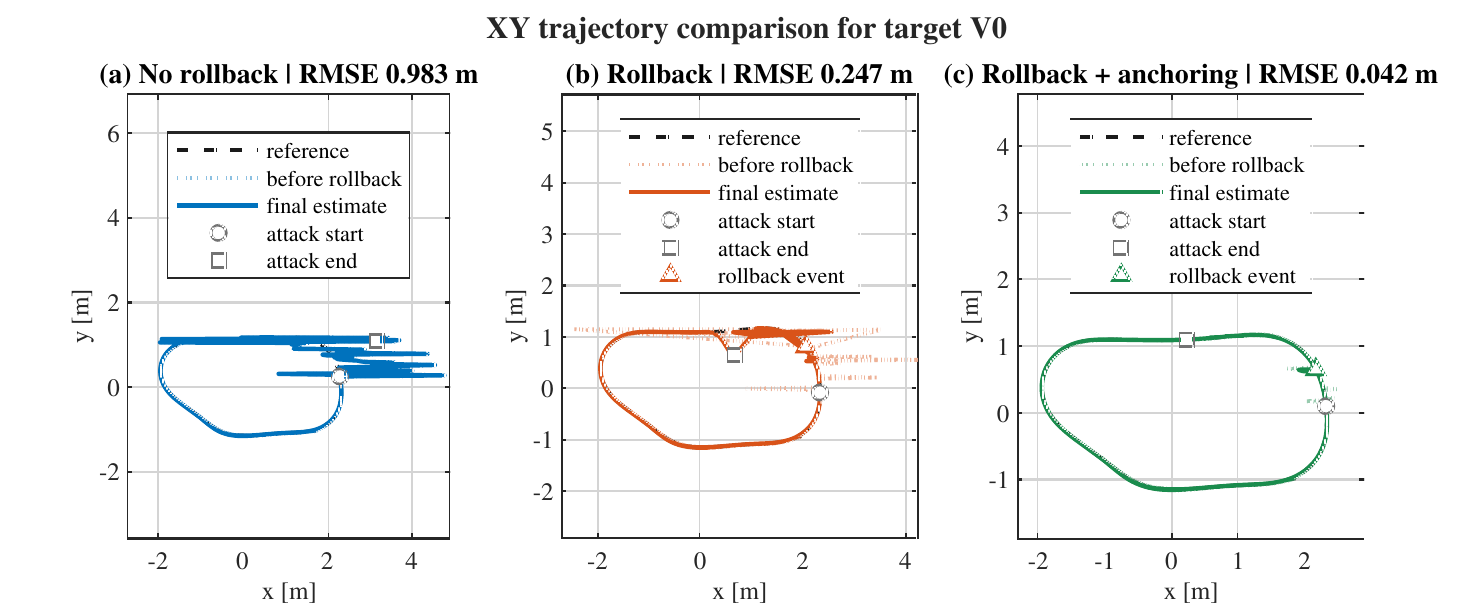
\includegraphics[width=\linewidth,height=0.57\textheight,keepaspectratio]{xy_case2_local.png}
    \end{column}
    \begin{column}{0.32\textwidth}
      \vspace{0.08cm}
      {\fontsize{9}{11}\selectfont No rollback}\par
      {\color{Ink}\fontsize{16}{18}\selectfont\bfseries 0.983 m}\par
      \vspace{0.09cm}
      {\fontsize{9}{11}\selectfont Rollback}\par
      {\color{Ink}\fontsize{16}{18}\selectfont\bfseries 0.247 m}\par
      \vspace{0.09cm}
      {\fontsize{9}{11}\selectfont Rollback plus accepted relative-pose anchoring}\par
      {\color{Accent}\fontsize{20}{22}\selectfont\bfseries 0.042 m}\par
      \vspace{0.10cm}
      {\color{Muted}\fontsize{8.1}{9.7}\selectfont Local-channel Case 2 RMSE. Correction reduces error 54.4\%; anchoring reduces it 75.2\%.}
    \end{column}
  \end{columns}
  \sourcefoot{Final trust-observer manuscript, QCar/LIMO rollback and anchoring results}
  \note{[Sources]\par
    \texttt{\detokenize{ch5/TRust_final/manuscript_v7_submit.tex}}, Rollback and anchoring results and Closed-loop trajectory diagnostics.\par
    Image converted from \texttt{\detokenize{ch5/TRust_final/img/XY_case2_local.eps}}.}
\end{frame}

% -----------------------------------------------------------------------------
\begin{frame}{Trust enables safe control degradation}
  \eyebrow{Approach 3 - control interaction}
  \begin{columns}[T,onlytextwidth]
    \begin{column}{0.58\textwidth}
      \centering
      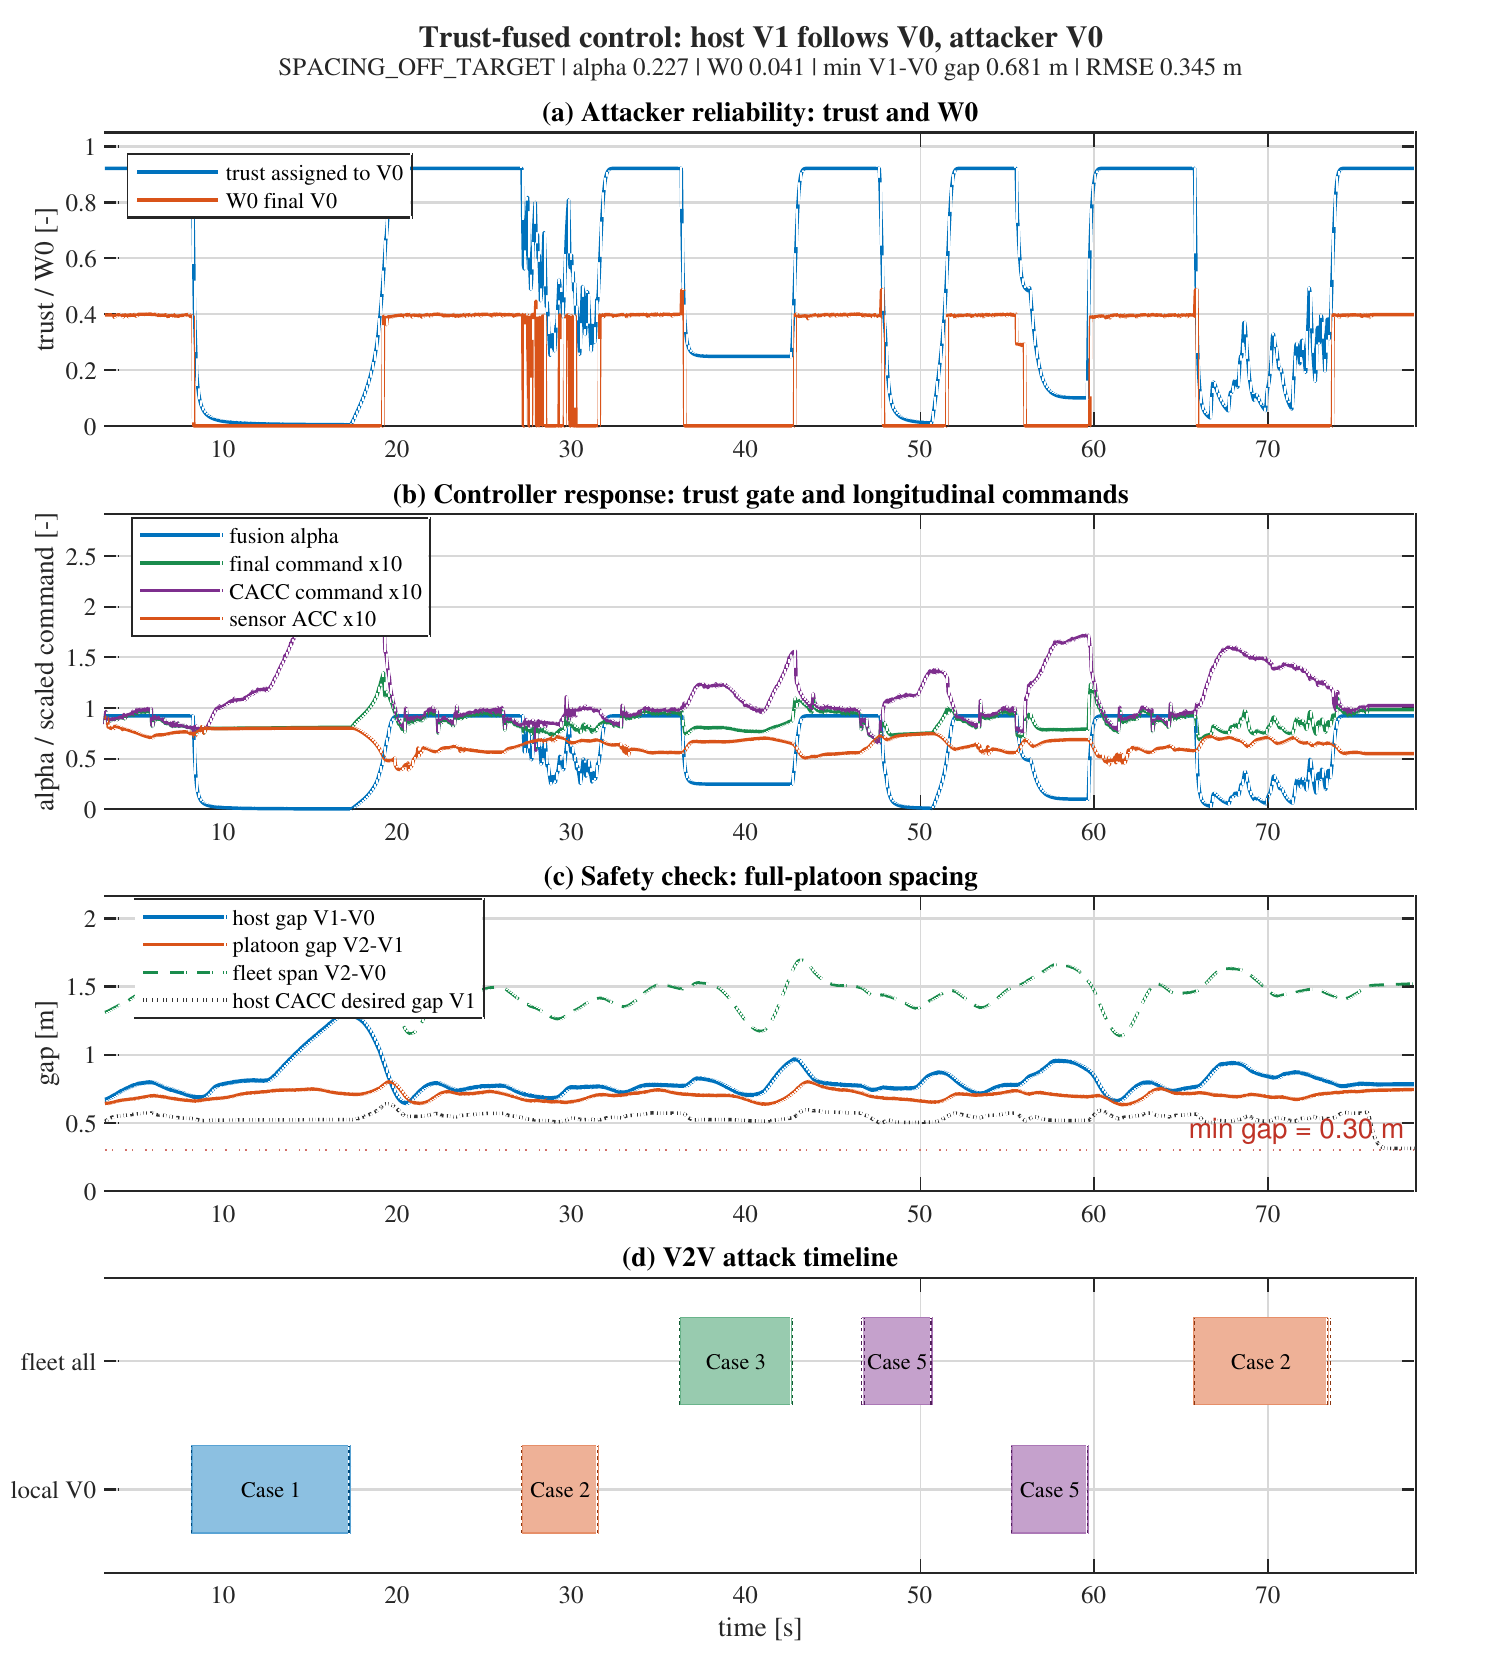
\includegraphics[height=0.63\textheight,width=\linewidth,keepaspectratio]{controller_fusion.png}
    \end{column}
    \begin{column}{0.37\textwidth}
      \quietmetric{$<0.05$}{Mean attacked-source observer weight}
      \vspace{0.25cm}
      \quietmetric{0.681 m}{V1 minimum path-projected gap}
      \vspace{0.25cm}
      \quietmetric{0.637 m}{V2 minimum path-projected gap}
      \vspace{0.25cm}
      \begin{beamercolorbox}[sep=0.15cm,wd=\linewidth]{block body}
        \fontsize{8.7}{10.4}\selectfont Both gaps remain above the study's 0.30 m reporting margin. The result is a feasibility check, not a formal full-footprint collision guarantee.
      \end{beamercolorbox}
    \end{column}
  \end{columns}
  \sourcefoot{Final trust-observer manuscript, trust-gated ACC/CACC metrics}
  \note{[Sources]\par
    \texttt{\detokenize{ch5/TRust_final/manuscript_v7_submit.tex}}, Distributed state estimation for platoon control and attack-window closed-loop metrics.\par
    Image converted from \texttt{\detokenize{ch5/TRust_final/img/controller_fusion.eps}}.}
\end{frame}

% -----------------------------------------------------------------------------
\begin{frame}{Tests reproduce the full operating loop}
  \eyebrow{Qualitative results}
  \begin{columns}[T,onlytextwidth]
    \begin{column}{0.62\textwidth}
      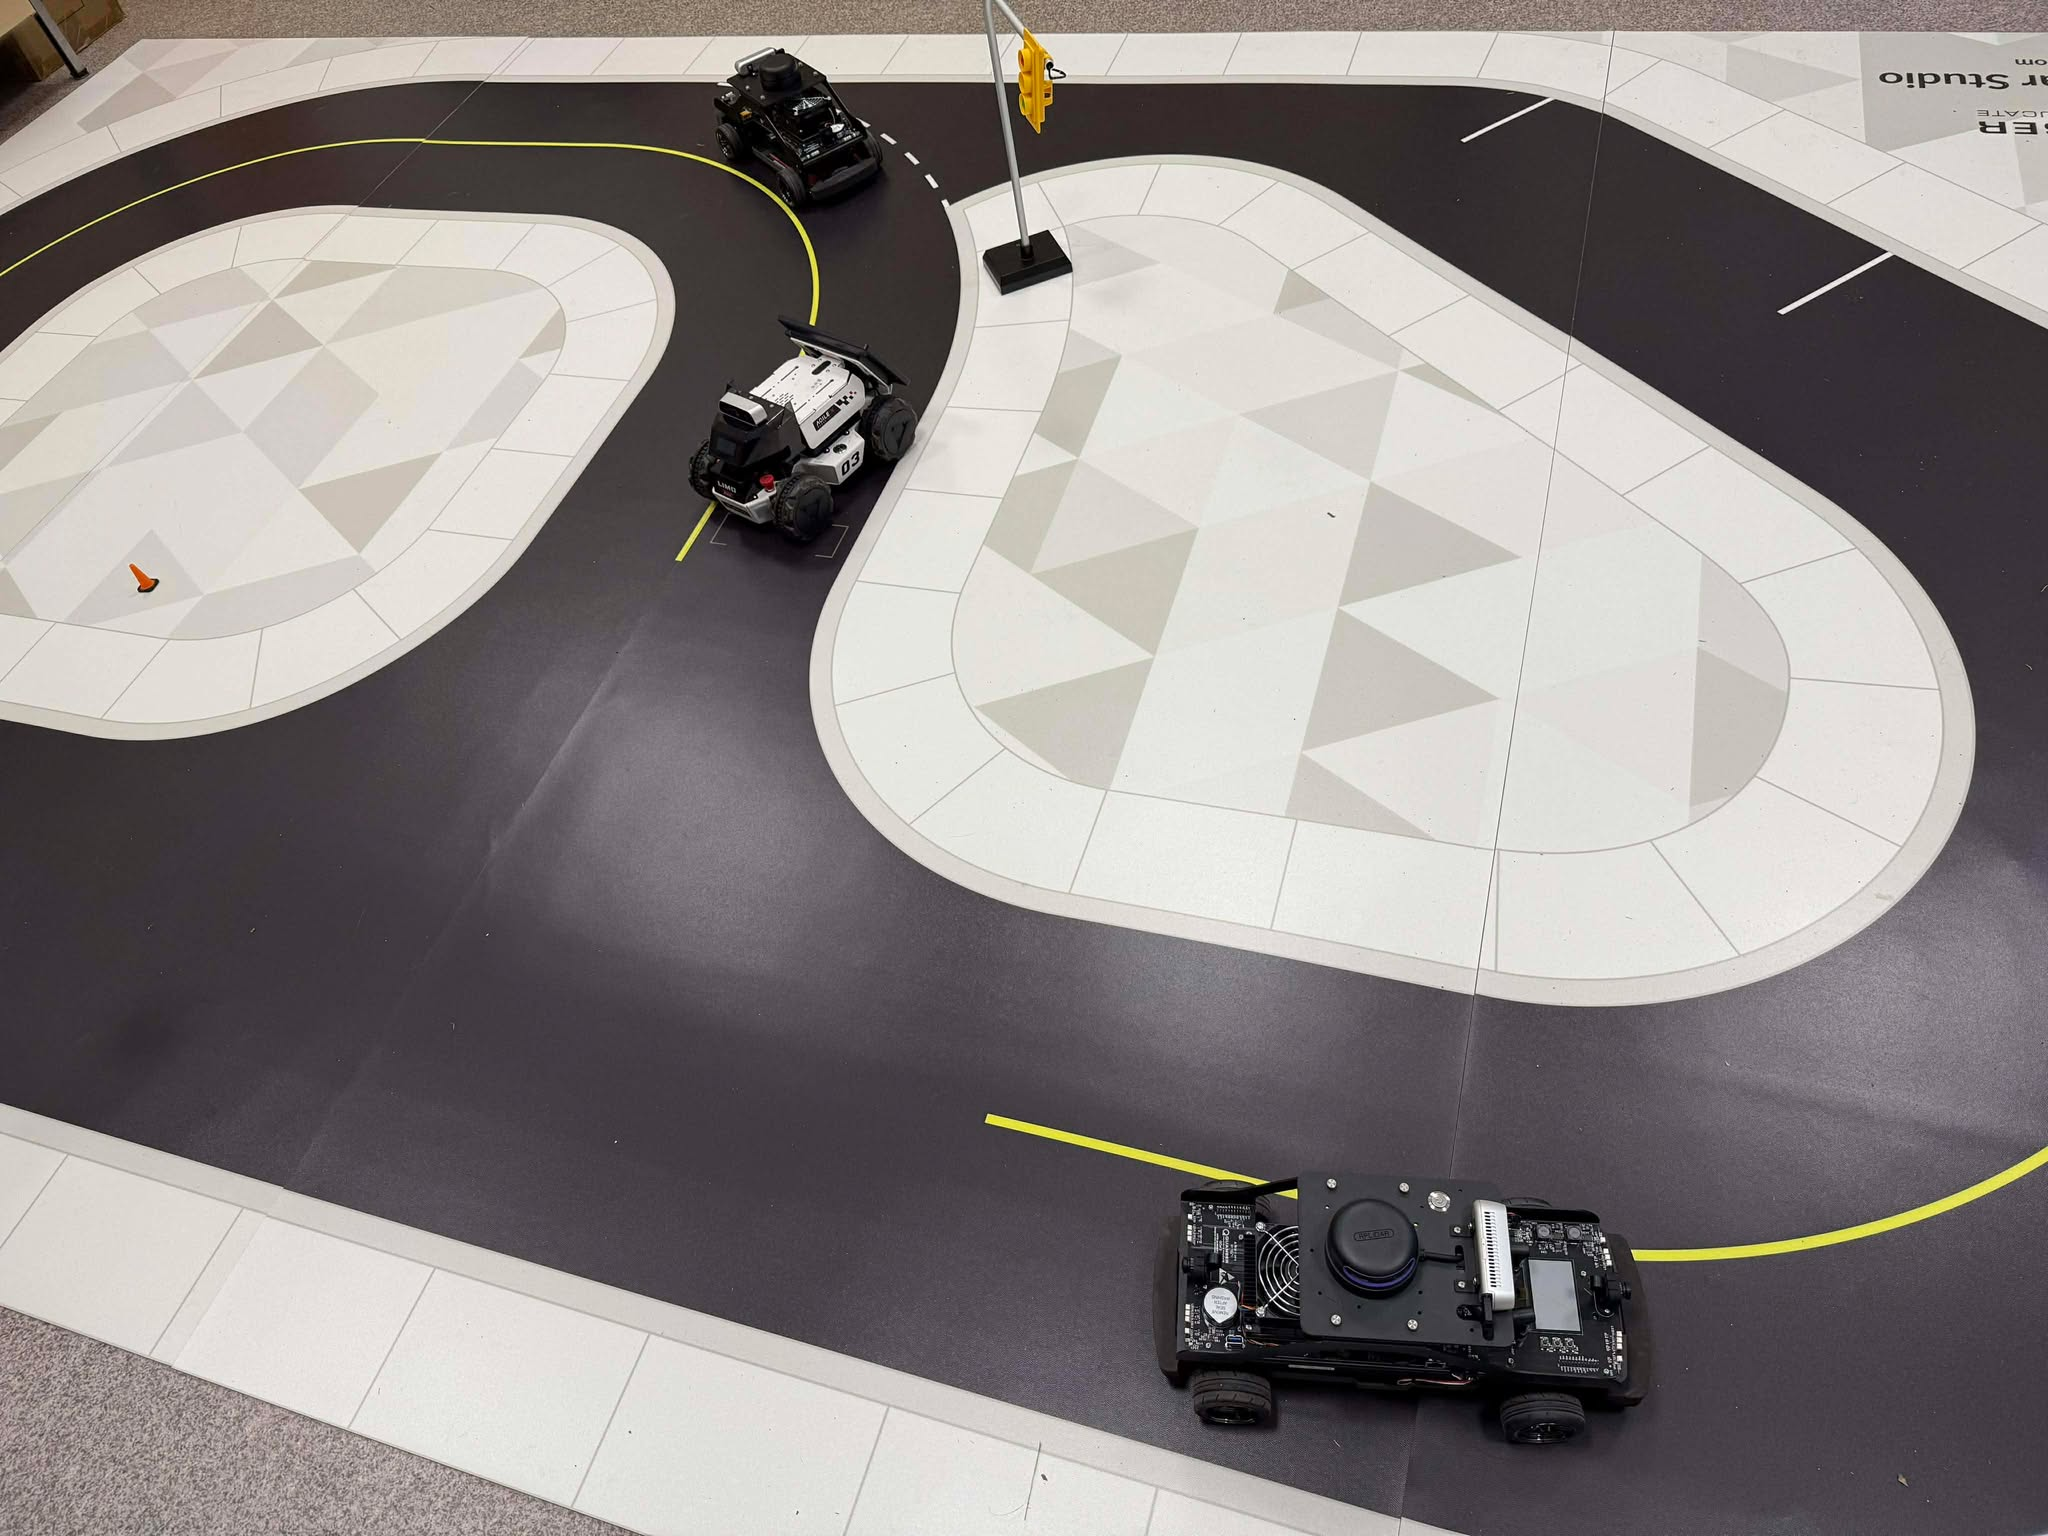
\includegraphics[width=\linewidth,height=0.39\textheight,keepaspectratio]{scale_model_track.jpg}\par
      \vspace{0.05cm}
      {\raggedright\color{Muted}\fontsize{7.5}{9}\selectfont Physical QCar/LIMO scale-model track\par}
    \end{column}
    \begin{column}{0.34\textwidth}
      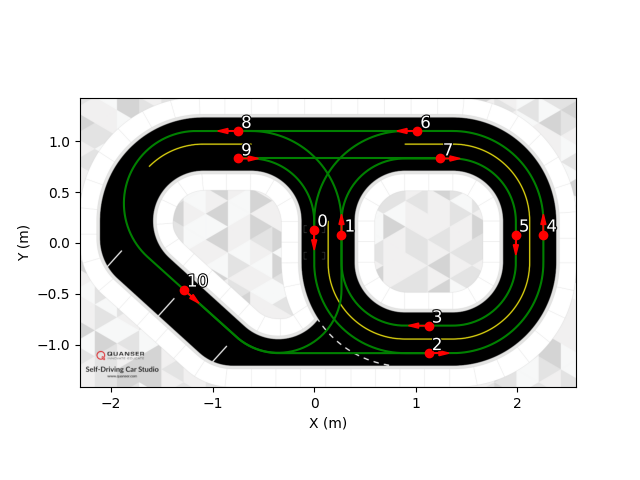
\includegraphics[width=\linewidth,height=0.17\textheight,keepaspectratio]{qlabs_map.png}\par
      \vspace{0.05cm}
      {\raggedright\color{Muted}\fontsize{7.5}{9}\selectfont QLabs trajectory and waypoint scenario\par}
      \vspace{0.06cm}
      {\fontsize{8.7}{10.4}\selectfont\bfseries One operating loop across both environments}\par
      \vspace{0.04cm}
      {\color{Muted}\fontsize{7.7}{9.2}\selectfont Same state, communication and control concepts; real packet timing; repeatable attacks and logged recovery.}
    \end{column}
  \end{columns}
  \sourcefoot{Thesis Chapter 6 and final manuscript QCar/LIMO implementation}
  \note{[Sources]\par
    Images: \texttt{\detokenize{ch6/fig/map_real.jpg}} and \texttt{\detokenize{ch6/fig/Figure_1.png}}.\par
    \texttt{\detokenize{ch6/ch6_main.tex}}, QLabs environment and experimental workflow.\par
    \texttt{\detokenize{ch5/TRust_final/manuscript_v7_submit.tex}}, QCar/LIMO platform validation.}
\end{frame}

% -----------------------------------------------------------------------------
\begin{frame}{The deployment platform is tangible}
  \eyebrow{Manufactured electronic board}
  \begin{columns}[T,onlytextwidth]
    \begin{column}{0.62\textwidth}
      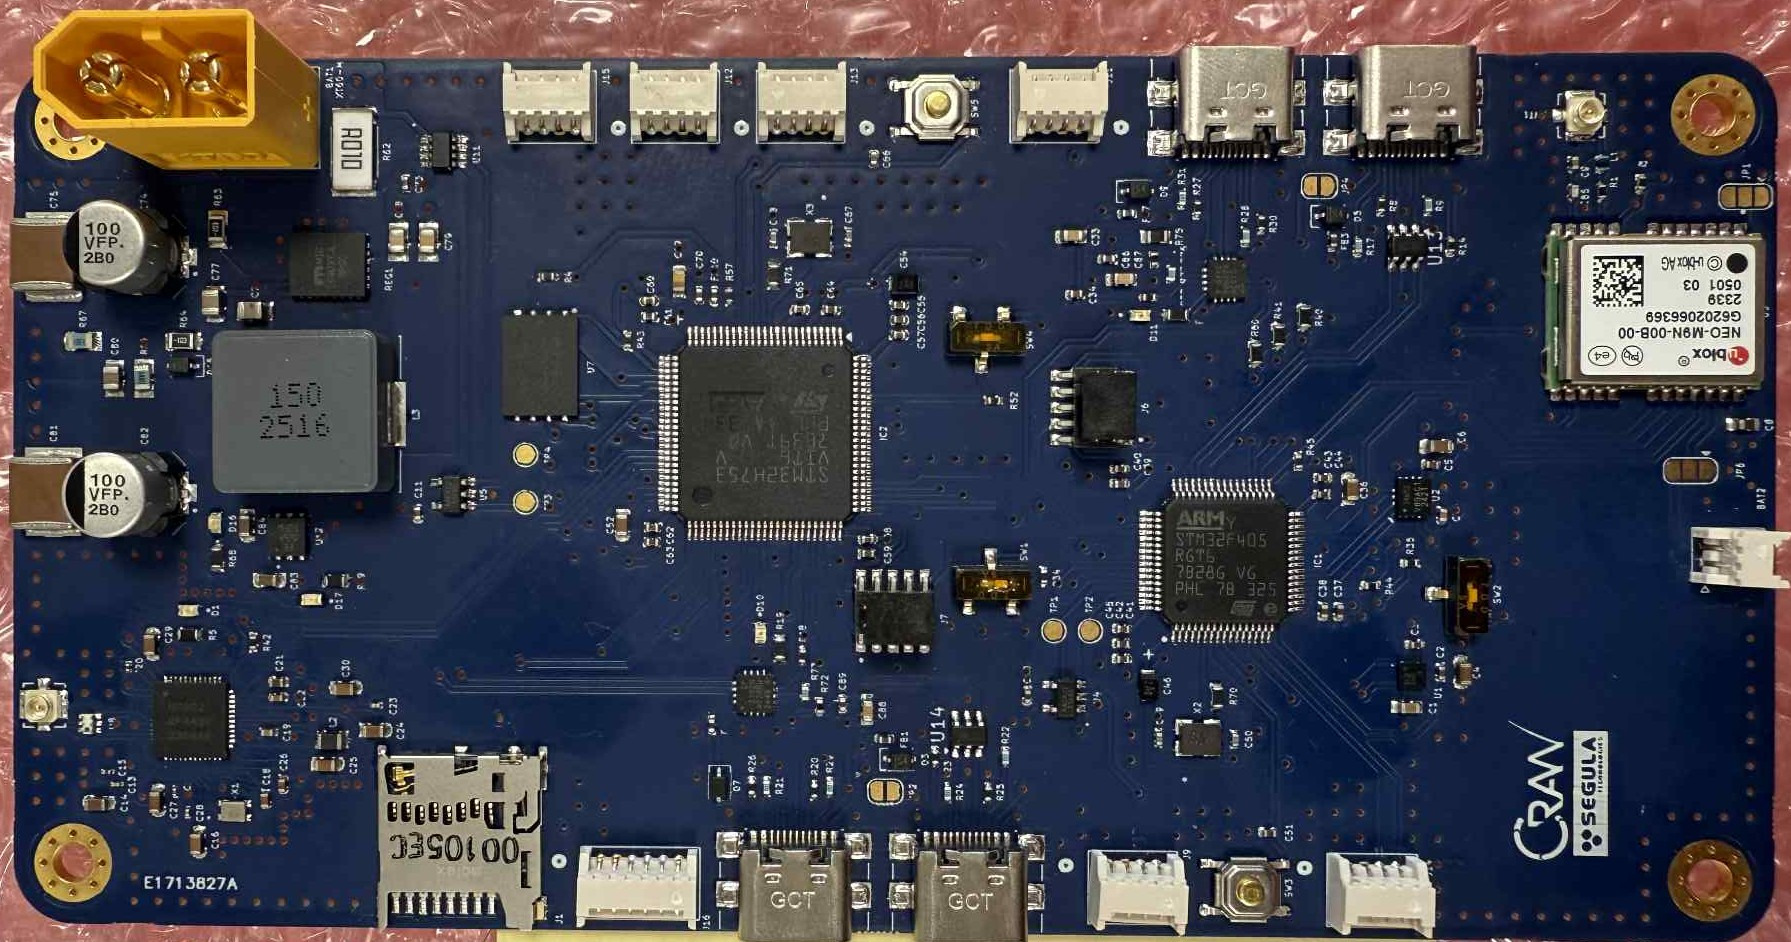
\includegraphics[width=\linewidth,height=0.52\textheight,keepaspectratio]{pcb_photo.jpg}
    \end{column}
    \begin{column}{0.34\textwidth}
      {\fontsize{9.3}{11.2}\selectfont
      \begin{itemize}
        \item Four-layer PCB with EMC-oriented grounding and power routing
        \item MCU/RTOS architecture targeting approximately 100 Hz estimation
        \item IMU, GNSS timing, Wi-Fi, storage and development interfaces
      \end{itemize}}
      \vspace{0.18cm}
      \begin{beamercolorbox}[sep=0.16cm,wd=\linewidth]{block body}
        \fontsize{8.5}{10.2}\selectfont\textbf{Bring-up evidence:} stable RTOS operation at 100 Hz, UART, GNSS acquisition and functional Wi-Fi 6 tests.
      \end{beamercolorbox}
    \end{column}
  \end{columns}
  \sourcefoot{Thesis Chapter 6, PCB design and first firmware validation tests}
  \note{[Sources]\par
    Image: \texttt{\detokenize{ch6/fig/cart_true.jpg}}.\par
    \texttt{\detokenize{ch6/ch6_main.tex}}, Architecture and PCB design; Firmware structure and first validation tests.}
\end{frame}

% -----------------------------------------------------------------------------
\begin{frame}{Aligned with standards; not certified}
  \eyebrow{Positioning versus state of the art}
  \begin{columns}[T,onlytextwidth]
    \begin{column}{0.47\textwidth}
      {\color{Good}\fontsize{12}{14}\selectfont\bfseries Transfer targets}\par
      \vspace{0.06cm}
      {\fontsize{8.8}{10.6}\selectfont
      \begin{itemize}
        \item 3GPP NR V2X / C-V2X radio
        \item SAE J2735 and C-ITS interoperability
        \item ISO/SAE 21434 lifecycle risk engineering
        \item UNECE R155 CSMS and ISO 26262 safe degradation
      \end{itemize}}
    \end{column}
    \begin{column}{0.47\textwidth}
      {\color{Warn}\fontsize{12}{14}\selectfont\bfseries Remaining industrialization}\par
      \vspace{0.06cm}
      {\fontsize{8.8}{10.6}\selectfont
      \begin{itemize}
        \item Secure boot, signed updates, keys and HSM
        \item Automotive EMC and environmental qualification
        \item Production V2X, CAN gateway and diagnostics
        \item Threat analysis, safety case, false positives and stealth attacks
      \end{itemize}}
    \end{column}
  \end{columns}
  \vspace{0.08cm}
  \begin{beamercolorbox}[sep=0.11cm,wd=\textwidth]{block body}
    \fontsize{8.7}{10.4}\selectfont\bfseries Research edge-estimation behind V2X - not a certified OBU or RSU.
  \end{beamercolorbox}
  \sourcefoot{Thesis Chapter 6; ISO/SAE 21434:2021; UNECE R155; ISO 26262 series}
  \note{[Sources]\par
    \texttt{\detokenize{ch6/ch6_main.tex}}, Architectural alignment with state of the art.\par
    ISO/SAE 21434:2021, Road vehicles - Cybersecurity engineering: https://www.iso.org/standard/70918.html\par
    UNECE UN Regulation No. 155: https://unece.org/transport/documents/2021/03/standards/un-regulation-no-155-cyber-security-and-cyber-security\par
    ISO 26262 series: https://www.iso.org/publication/PUB200262.html}
\end{frame}

% -----------------------------------------------------------------------------
\begin{frame}{Value comes from portable resilience}
  \eyebrow{Economic relevance}
  \vspace{0.05cm}
  \begin{columns}[T,onlytextwidth]
    \begin{column}{0.30\textwidth}
      \stepnumber{01}\par\vspace{0.12cm}
      {\fontsize{13}{15}\selectfont\bfseries Reuse across platforms}\par
      \vspace{0.15cm}
      {\color{Muted}\fontsize{8.8}{10.6}\selectfont A portable edge node separates estimation and trust services from a specific vehicle computer or sensor stack.}
    \end{column}
    \begin{column}{0.30\textwidth}
      \stepnumber{02}\par\vspace{0.12cm}
      {\fontsize{13}{15}\selectfont\bfseries Protect cooperation}\par
      \vspace{0.15cm}
      {\color{Muted}\fontsize{8.8}{10.6}\selectfont Unreliable cooperative data can be isolated while local sensing and local control remain available.}
    \end{column}
    \begin{column}{0.30\textwidth}
      \stepnumber{03}\par\vspace{0.12cm}
      {\fontsize{13}{15}\selectfont\bfseries Shorten evidence loops}\par
      \vspace{0.15cm}
      {\color{Muted}\fontsize{8.8}{10.6}\selectfont Digital-twin reuse, configurable attacks and onboard logs accelerate testing and root-cause analysis.}
    \end{column}
  \end{columns}
  \vspace{0.20cm}
  \begin{beamercolorbox}[sep=0.12cm,wd=\textwidth]{block body}
    \fontsize{9.2}{11}\selectfont\textbf{Economic hypothesis for the pilot:} lower integration effort and fewer attack-induced degradations than controller-only filtering or platform-specific implementations. Quantified ROI still requires vehicle-program data.
  \end{beamercolorbox}
  \sourcefoot{Thesis Chapter 6, board motivation and virtual-to-real workflow}
  \note{[Sources]\par
    \texttt{\detokenize{ch6/ch6_main.tex}}, board motivation and design objectives; experimental workflow; traceability and reproducibility.\par
    The economic statement is explicitly framed as a hypothesis requiring pilot data, not a measured financial result.}
\end{frame}

% -----------------------------------------------------------------------------
\begin{frame}{A shadow-mode pilot is the next gate}
  \eyebrow{Recommended continuation}
  \begin{columns}[T,onlytextwidth]
    \begin{column}{0.56\textwidth}
      {\fontsize{8.3}{10}\selectfont
      \begin{tabular}{@{}p{0.10\linewidth}>{\RaggedRight\arraybackslash}p{0.84\linewidth}@{}}
        \stepnumber{01} & \textbf{Connect} production V2X and the target vehicle bus. \\[0.05cm]
        \stepnumber{02} & \textbf{Run monitor-only}; log trust,\newline rejection and recovery. \\[0.05cm]
        \stepnumber{03} & \textbf{Measure} detection, false positives, timing and memory. \\[0.05cm]
        \stepnumber{04} & \textbf{Authorize CACC-to-ACC fallback} only after the gates pass. \\
      \end{tabular}}
    \end{column}
    \begin{column}{0.39\textwidth}
      \begin{beamercolorbox}[sep=0.13cm,wd=\linewidth]{block body}
        {\fontsize{11.5}{13.5}\selectfont\bfseries Go / no-go evidence}\par
        \vspace{0.06cm}
        {\fontsize{8.2}{9.8}\selectfont\begin{itemize}
          \item Timing / compute budget
          \item Detection and false positives
          \item Delay / dropout / stealth coverage
          \item EMC, power and interfaces
          \item Vehicle integration effort
        \end{itemize}}
      \end{beamercolorbox}
    \end{column}
  \end{columns}
  \vspace{0.05cm}
  {\fontsize{8.2}{9.8}\selectfont\bfseries Decision: pursue when a vehicle program provides bus access and a cooperative-driving use case.}
  \sourcefoot{Thesis Chapter 6, staged integration roadmap and future validation axes}
  \note{[Sources]\par
    \texttt{\detokenize{ch6/ch6_main.tex}}, Integration roadmap with thesis algorithms and future optimization/stress-test axes.\par
    Recommendation is an inference from the documented monitoring-first roadmap and current maturity.}
\end{frame}

\end{document}
